\subsection{تخمین پارامتر کانال پیچ}
برای اصلاح پارامترها پیچ چندین آزمایش انجام شد و با استفاده از خروجیآزمایش و جعبه‌ابزاز
\lr{Parameter Estimator}
پارامترها اصلاح شدند.
برای آزمایش پیچ هر یک از موتورهای یک و سه  با دور مختلف شروع به حرکت کردند و خروجیسنسور داده برداری شد. سپس، مدل و پارامترهای داده برداری شده به جعبه‌ابزار
\lr{Parameter Estimator}
داده شد. نتایج آزمایش‌های کانال پیچ بعد از اصلاح پارامترها در شکل‌های
(\ref{pitch_ps1}, \ref{pitch_ps2}, \ref{pitch_ps3})
آورده شده است.

\begin{figure}[H]
	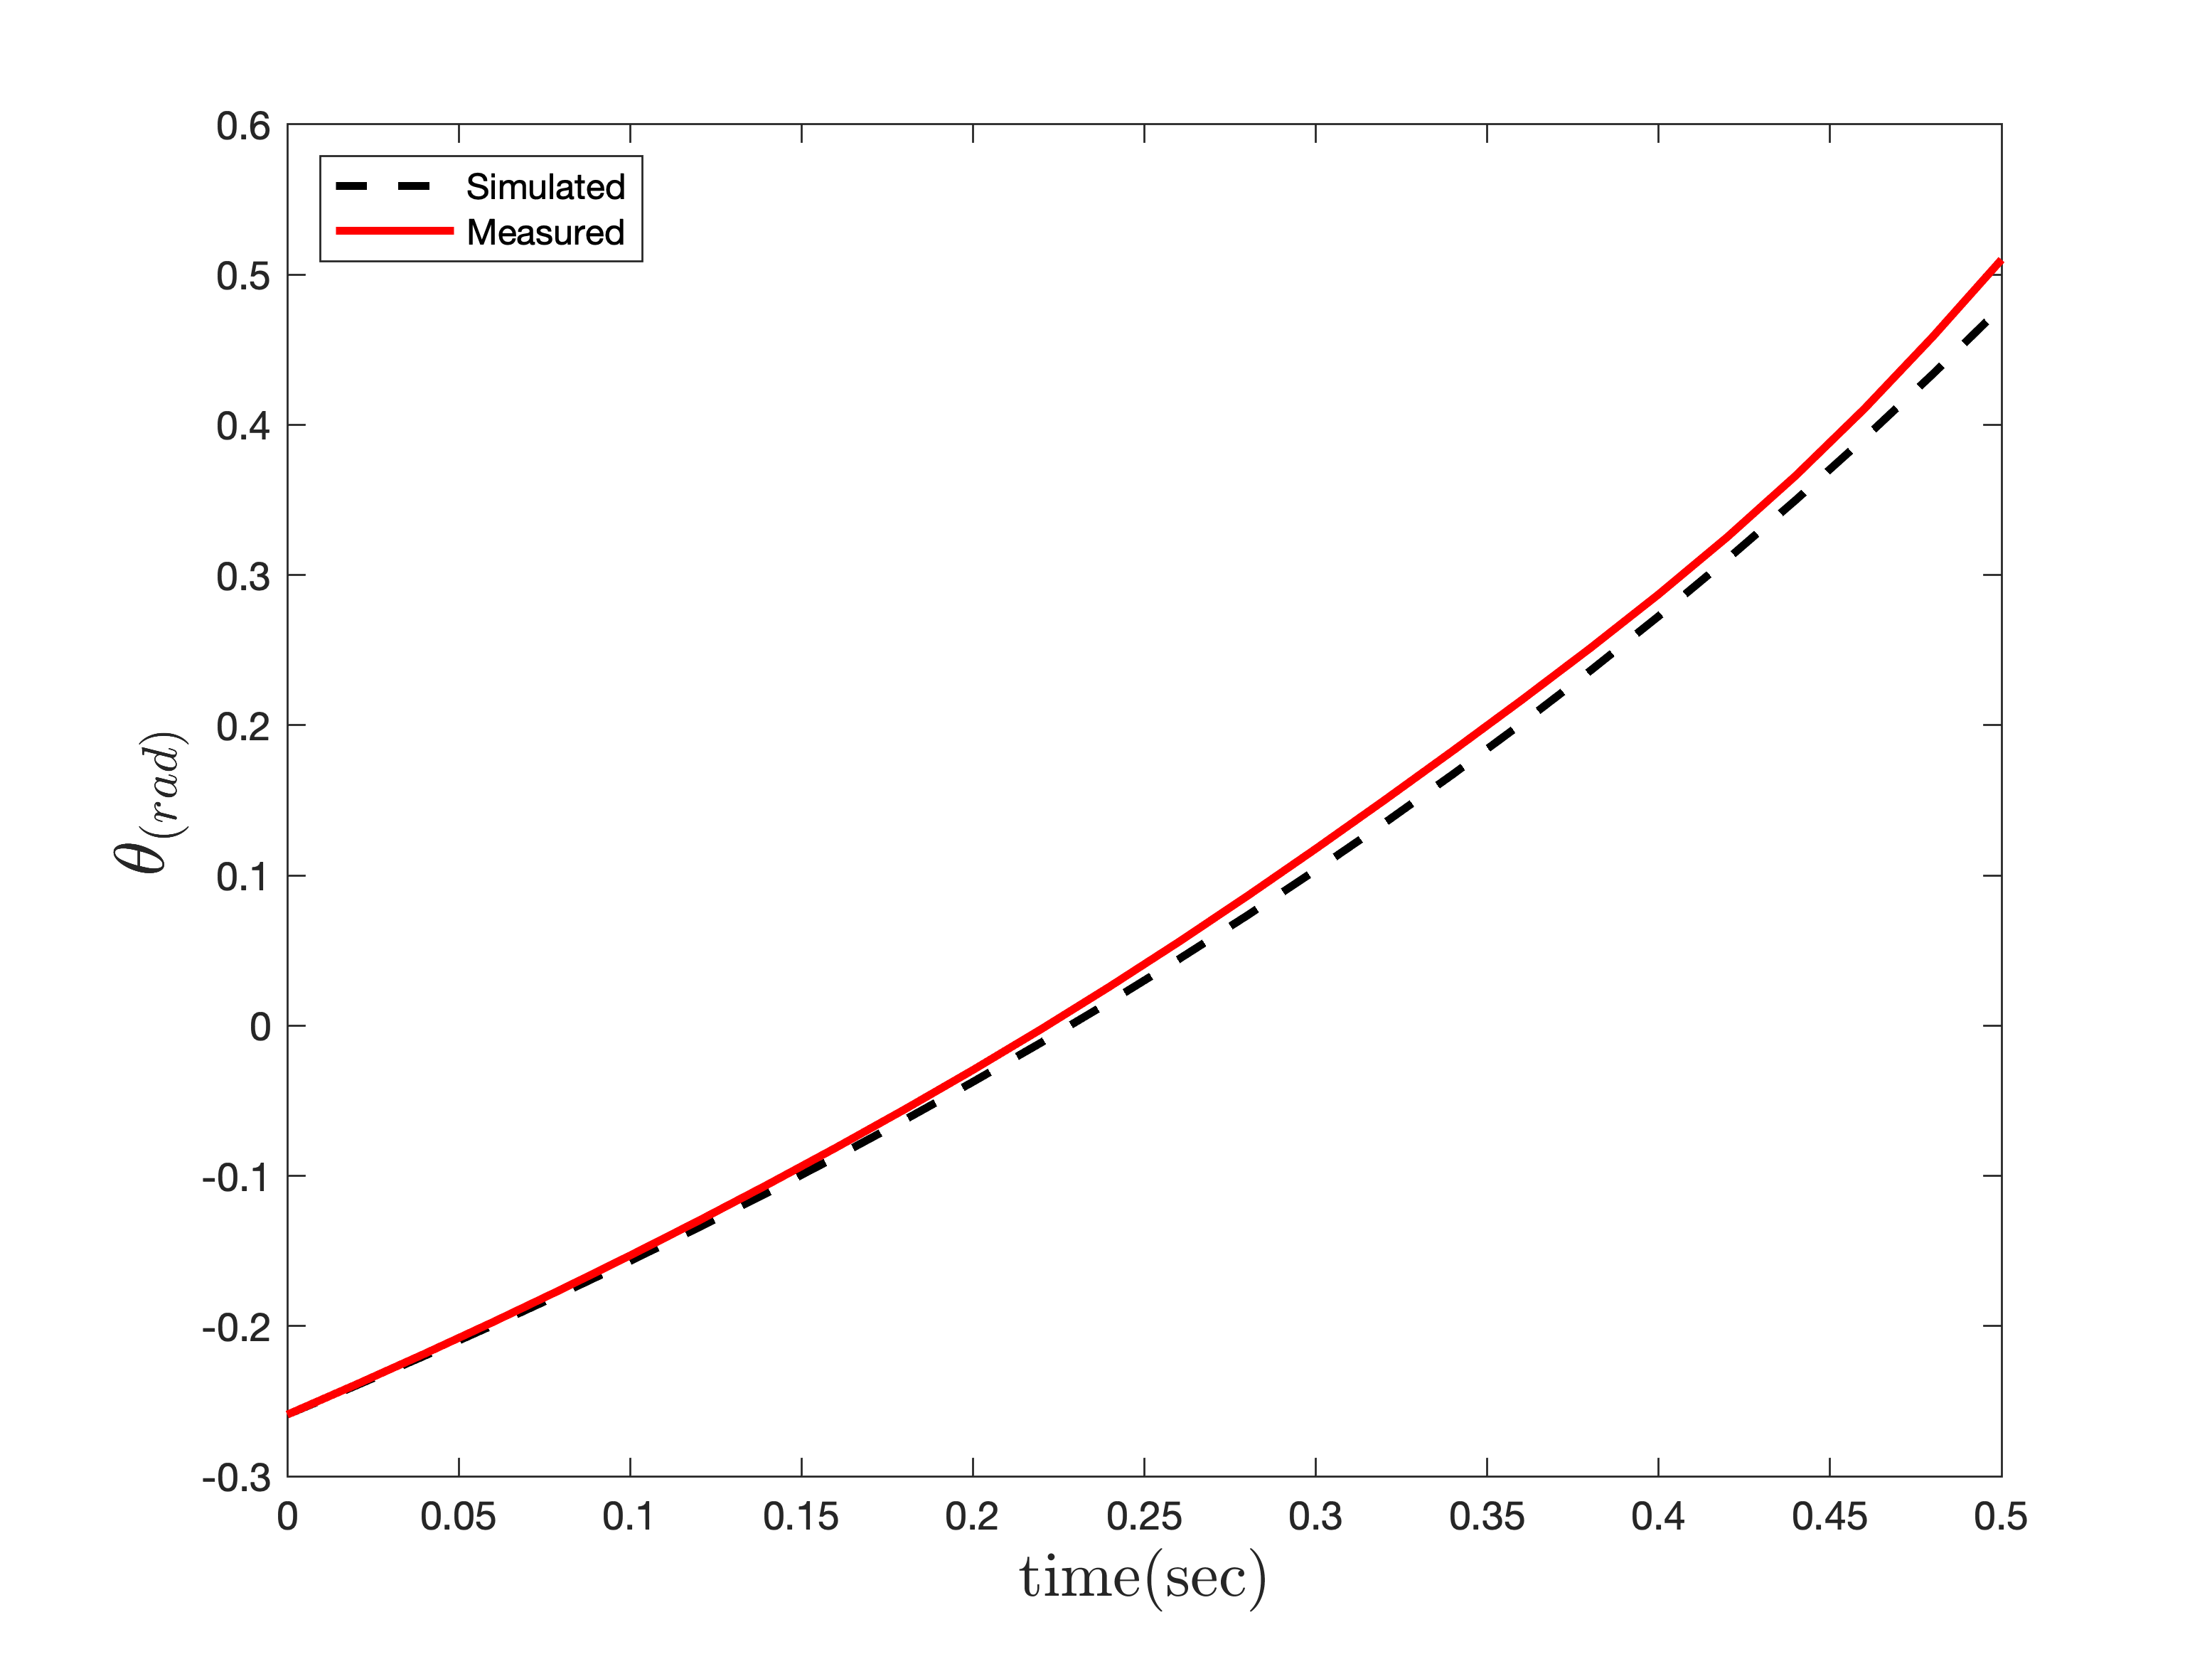
\includegraphics[width=12cm]{../../Figures/RCP/pitch_parameter_estimation/RCP_pitch_S1.png}
	\centering
	\caption{مقايسه خروجی‌های آزمايش اول و خروجیشبیه‌سازی پس از تخمین پارامترهای کانال پیچ}
	\label{pitch_ps1}
\end{figure}
\begin{figure}[H]
	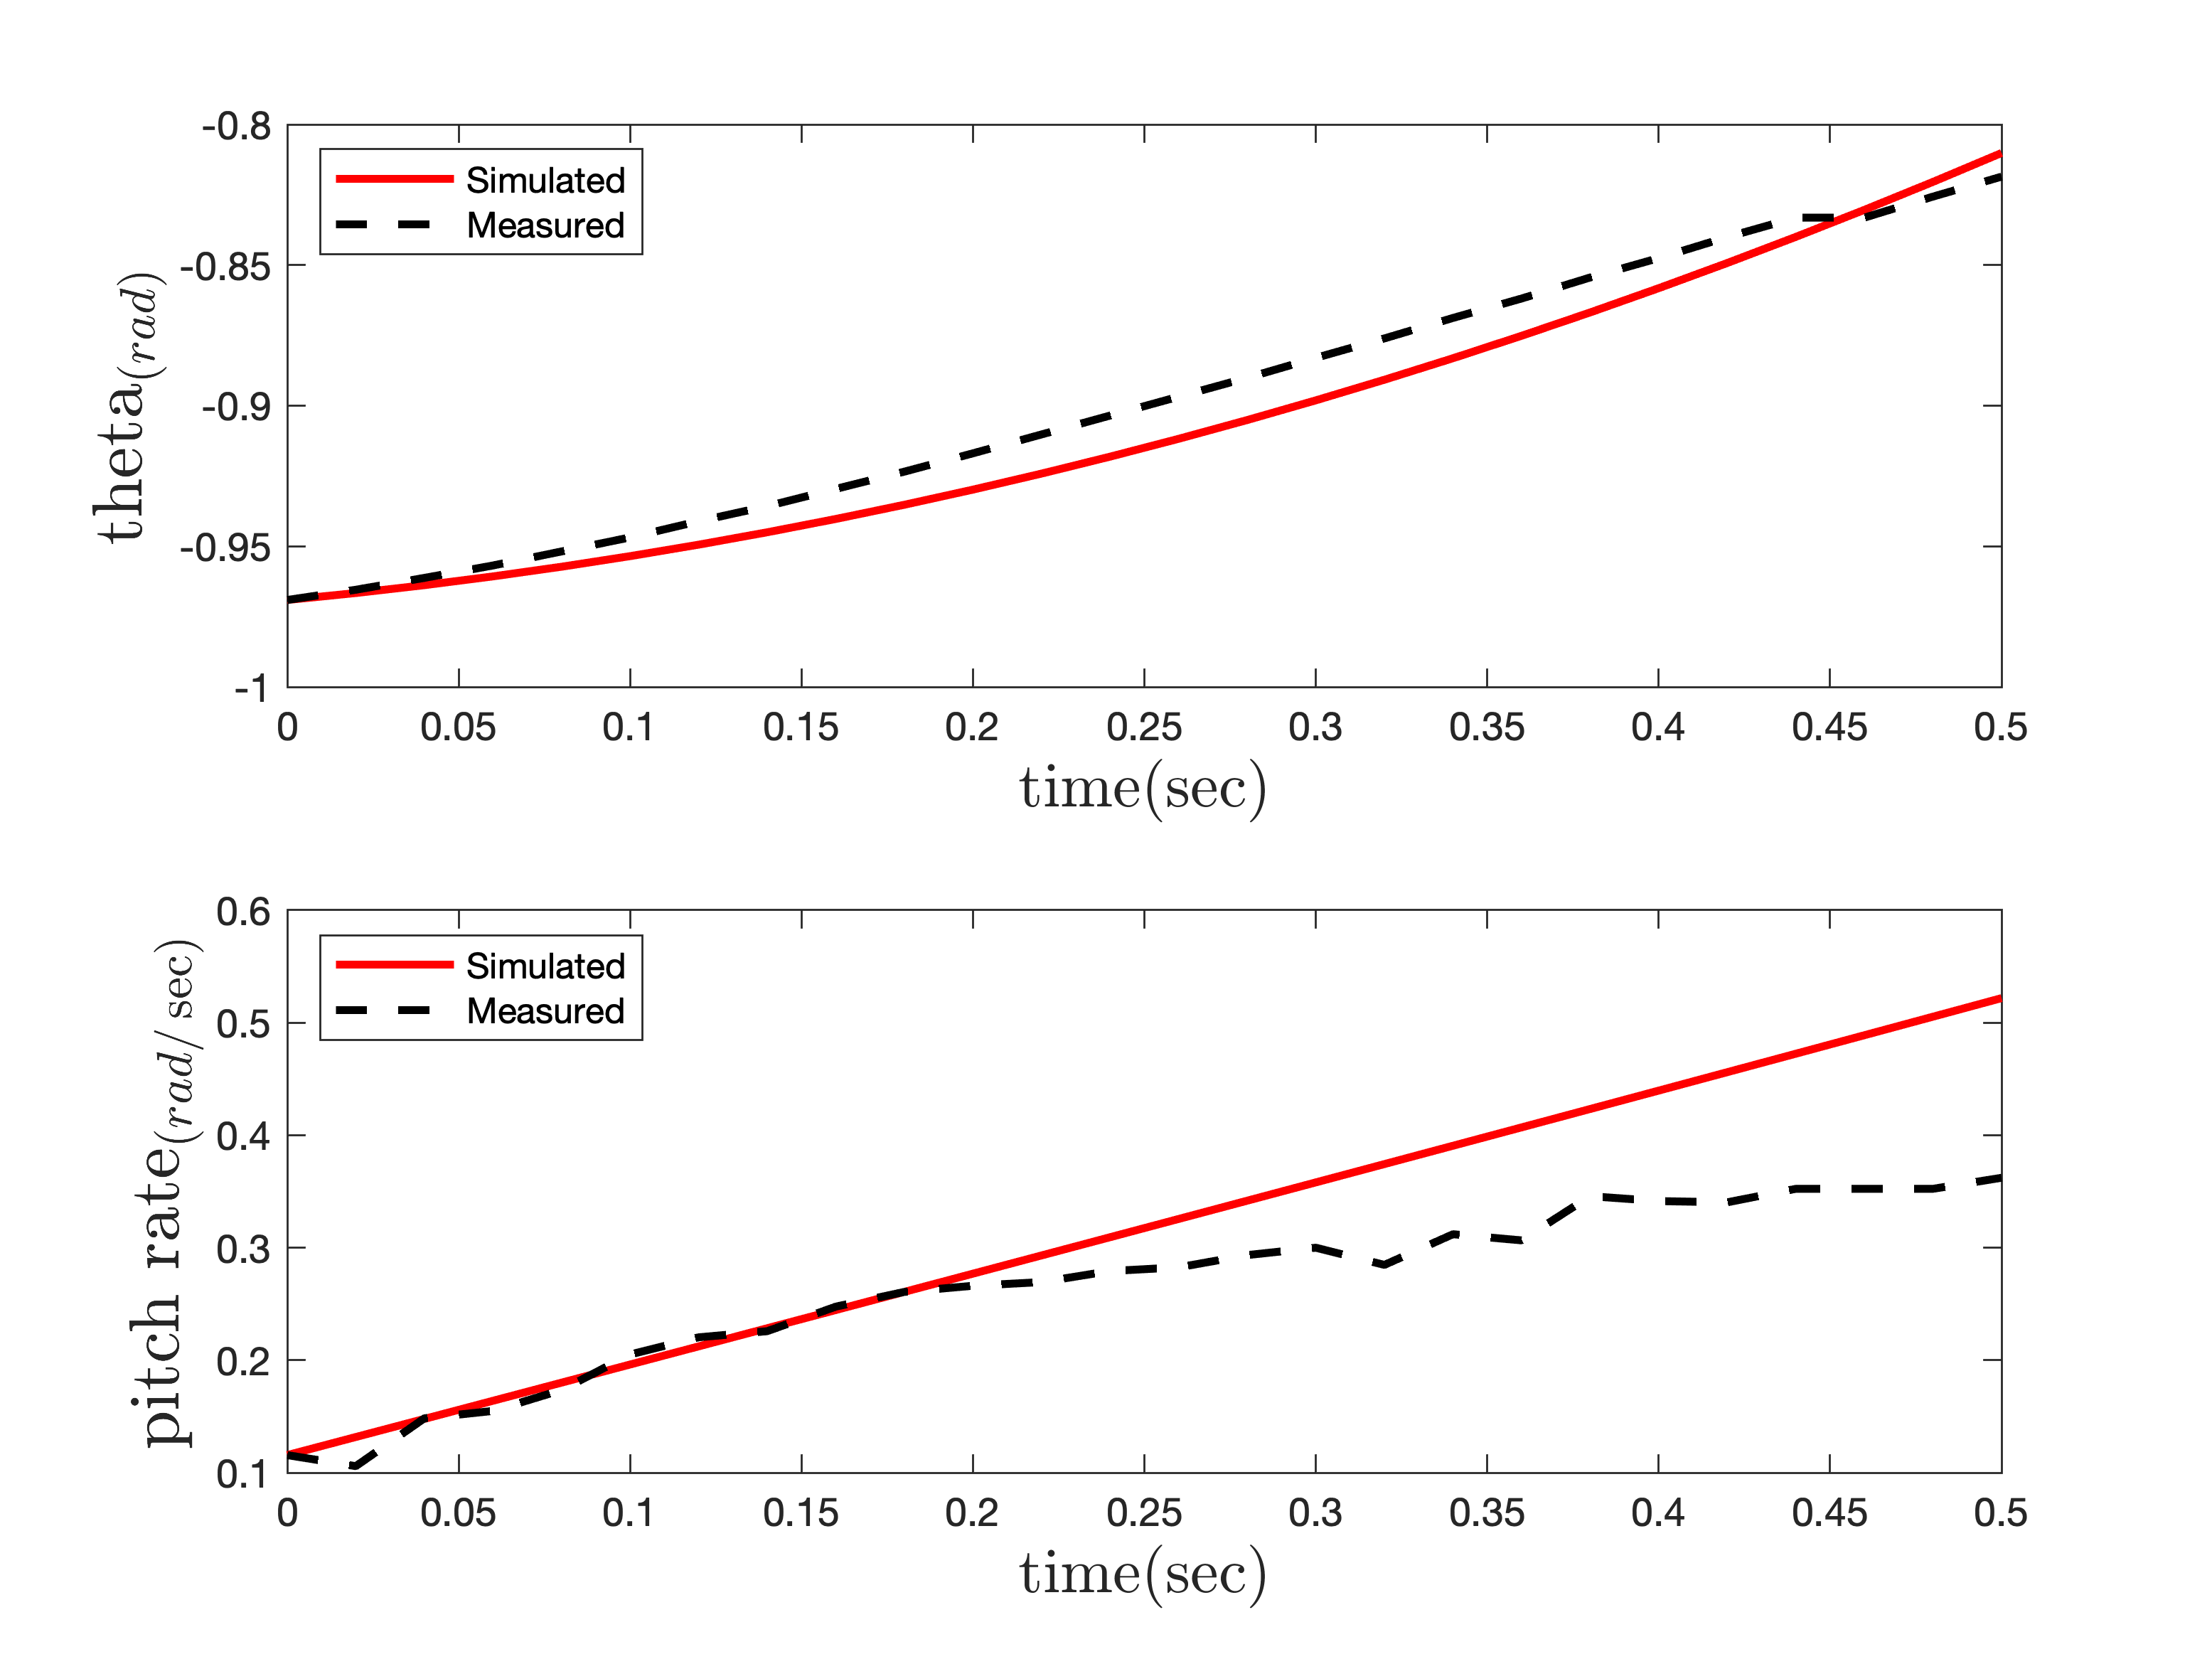
\includegraphics[width=12cm]{../../Figures/RCP/pitch_parameter_estimation/RCP_pitch_S2.png}
	\centering
	\caption{مقايسه خروجی‌های آزمايش دوم و خروجیشبیه‌سازی پس از تخمین پارامترهای کانال پیچ}
	\label{pitch_ps2}
\end{figure}
\begin{figure}[H]
	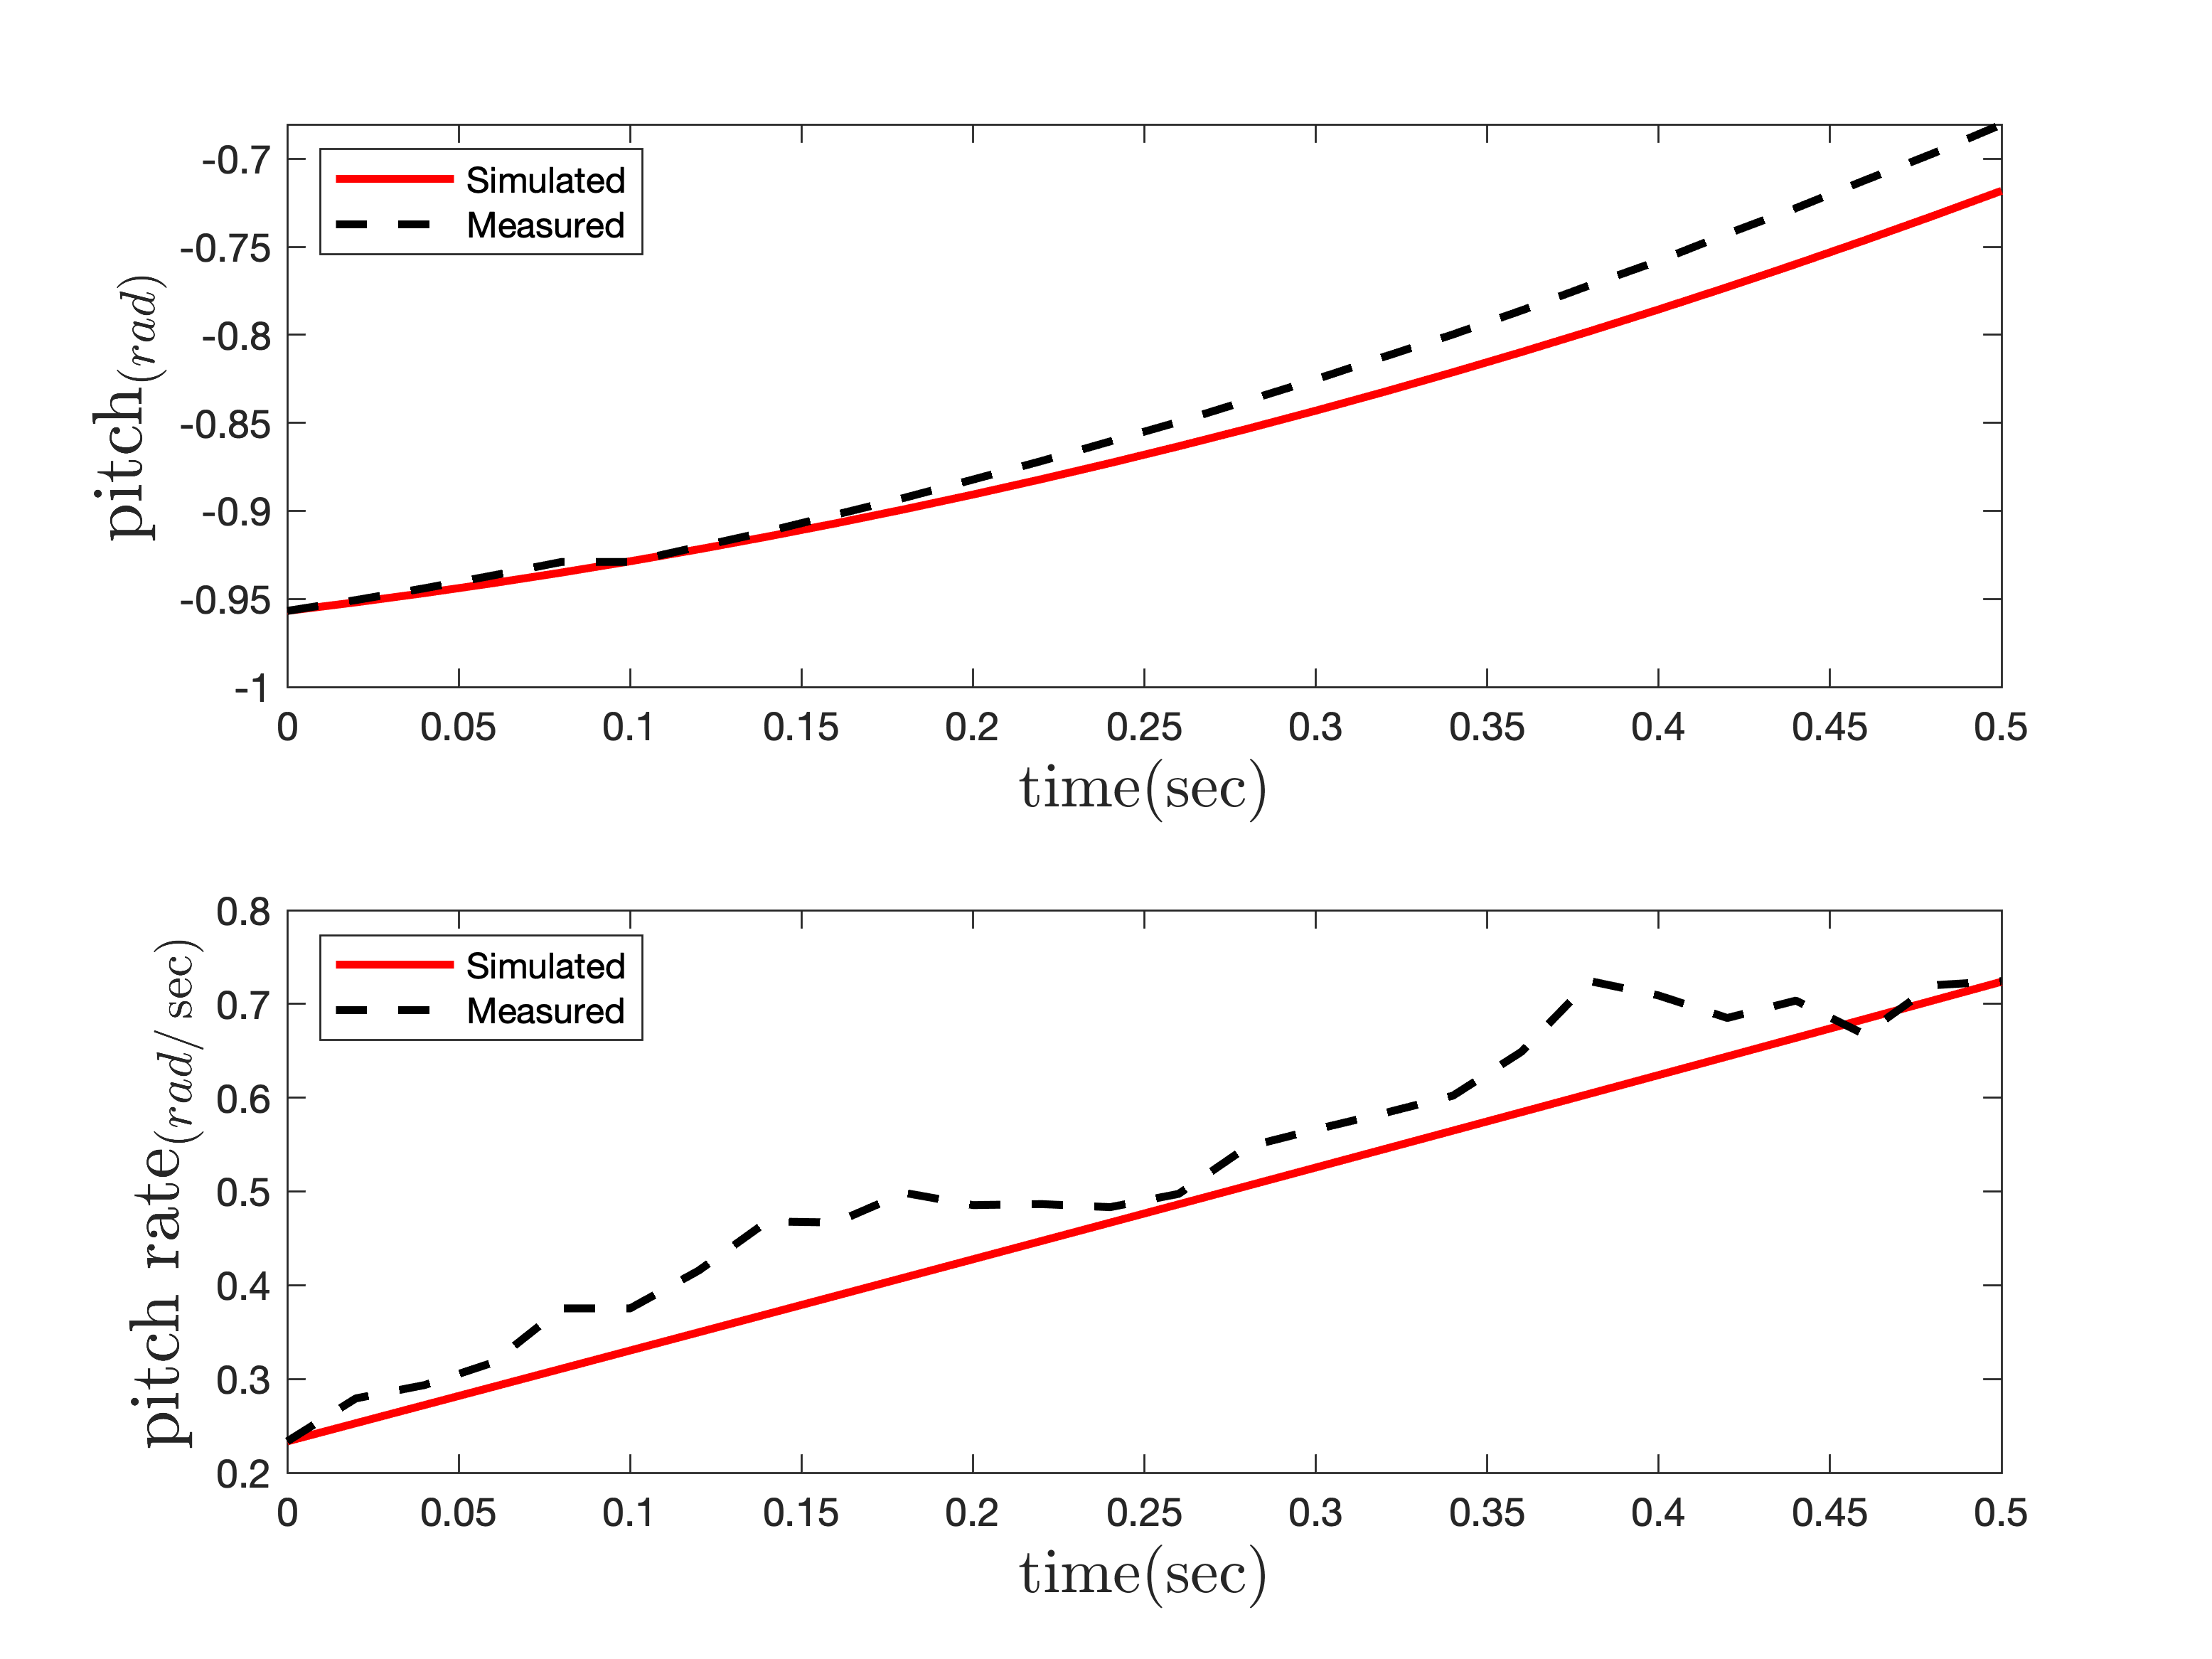
\includegraphics[width=12cm]{../../Figures/RCP/pitch_parameter_estimation/RCP_pitch_S3.png}
	\centering
	\caption{مقايسه خروجی‌های آزمايش سوم و خروجیشبیه‌سازی پس از تخمین پارامترهای کانال پیچ}
	\label{pitch_ps3}
\end{figure}